\documentclass[../../../include/open-logic-section]{subfiles}

\begin{document}

\olfileid{sth}{ordinals}{idea}	
\olsection{The General Idea of an Ordinal}

Consider the natural numbers, in their usual order:
\begin{center}
	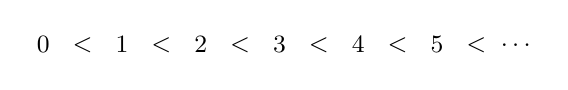
\begin{tikzpicture}
	\foreach \x/\xtext in {0, 1, 2, 3, 4, 5}
	{
		\node (\x a) at (\x, 1) {\small{$\x$}};
		\node (\x a) at (\x.5, 1) {\small{$<$}};
	}
	\node (ldots) at (6, 1) {\small{$\ldots$}};
	\end{tikzpicture}
\end{center}
We call this, in the jargon, an $\omega$-sequence. And indeed, this
general ordering is mirrored in our initial construction of the stages
of the set hierarchy. But, now suppose we move $0$ to the end of this
sequence, so that it comes after all the other numbers:
\begin{center}
	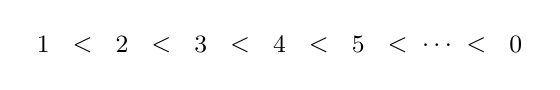
\begin{tikzpicture}
	\foreach \x/\xtext in {1, 2, 3, 4, 5}
	{
		\node (\x a) at (\x, 1) {\small{$\x$}};
		\node (\x a) at (\x.5, 1) {\small{$<$}};
	}
	\node (ldots) at (6, 1) {\small{$\ldots$}};
	\node (bea) at (6.5, 1) {\small{$<$}};
	\node (noa) at (7, 1) {\small{$0$}};
	\end{tikzpicture}
\end{center}
We have the same entities here, but ordered in a fundamentally
different way: our first ordering had no last element; our new
ordering does. Indeed, our new ordering consists of an
$\omega$-sequence of entities ($1, 2, 3, 4, 5, \ldots$), followed by
another entity. It will be an $\omega+1$-sequence.

We can generate even more types of ordering, using just these
entities. For example, consider all the even numbers (in their natural
order) followed by all the odd numbers (in their natural order):
\begin{center}
	\begin{tikzpicture}
	\node(a1) at (1,1) {\small{$0$}};
	\node(a2) at (1.5,1) {\small{$<$}};
	\node(a3) at (2,1) {\small{$2$}};
	\node(a4) at (2.5,1) {\small{$<$}};
	\node(a5) at (3,1) {\small{$4$}};
	\node(a6) at (3.5,1) {\small{$<$}};
	\node(dots) at (4,1) {\small{$\ldots$}};
	\node(aaoe) at (4.5,1) {\small{$<$}};
	\node(b1) at (5,1) {\small{$1$}};
	\node(b2) at (5.5,1) {\small{$<$}};
	\node(b3) at (6,1) {\small{$3$}};
	\node(b4) at (6.5,1) {\small{$<$}};
	\node(b5) at (7,1) {\small{$\ldots$}};
	\end{tikzpicture}
\end{center}
This is an $\omega$-sequence followed by another $\omega$-sequence; an
$\omega+\omega$-sequence. 

Well, we can keep going. But what we would like is a general way to
understand this talk about \emph{orderings}. 

\end{document}